\documentclass[12pt,letterpaper]{article}
\usepackage[utf8]{inputenc}
\usepackage{amsmath}
\usepackage{amsfonts}
\usepackage{amssymb}
\usepackage{graphicx}
\usepackage[left=2cm,right=2cm,top=2cm,bottom=2cm]{geometry}

\usepackage{subfigure}

\author{Tanmoy Sanyal}
\title{CMPSC 240A HW-3 Report}

\begin{document}
\maketitle

\section*{Brief code summary}
\noindent The code follows the logic outlined in the description of the assignment. \texttt{rec\_cilkified} works by divide and conquer. The arrays are divided into two (not always equal) parts recursively and their individual dot products are summed up, until a certain threshold (COARSENESS) is reached. After that point, the dot products are done in a simple serial for loop. \texttt{cilk\_spawn} is used in the splitting so that the recursive function calls are spawned off in different threads. \texttt{loop\_cilkified} works in a similar way, but instead of recursion, it splits the arrays into chunks of length = COARSENESS and then these chunks are "dot"-ed individually and added up. \texttt{hyperobject\_cilkified} simply uses the hyperobject construct of cilk++ and it takes care of everything.\\

\noindent For all the scaling experiments, I have assumed that the number of threads is the same as the number of cores (and set using the CILK\_NWORKERS environment variable). Further, since these are scaling experiments, cases with incorrect results have also been included. 

\section*{Scaling with size of array}
\noindent For this experiment, the COARSENESS was chosen to be 50, and was run on all 24 cores of a single Comet compute node. The array sizes were varied from $10^4$ to $10^{10}$. However, the sequential algorithm run-time for sizes below $10^6$ was almost negligible, and reported as 0.
%
\begin{figure}[h]
\centering
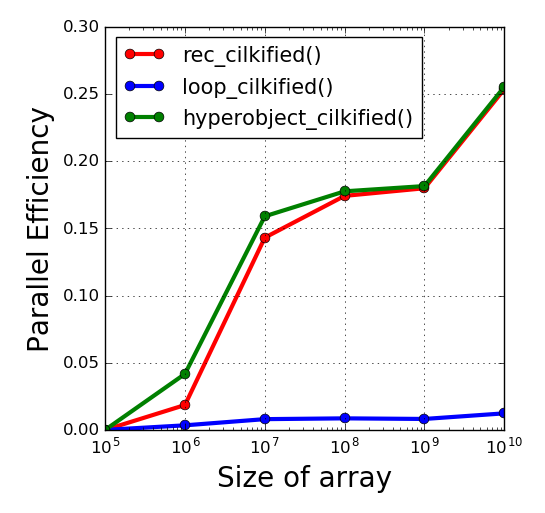
\includegraphics[scale=0.45]{arrsize_scaling.png}
\caption{Parallel efficiency vs array size, NCores = 24, COARSENESS = 50}
\end{figure}
%
\section*{Scaling with number of cores}
\noindent For this experiment, the array size was fixed at $10^6$ and COARSENESS was maintained at 50. The number of cores was varied from 1 to 64 in powers of 2. Note that the work ($t_1$) for this experiment is not the runtime of the sequential function \texttt{std::inner\_product}, but the time obtained with 1 core and CILK\_NWORKERS =1 .(For 32 and 64 cores, I use 16 cores per compute node and multiple nodes).
%
\begin{figure}[h]
\centering
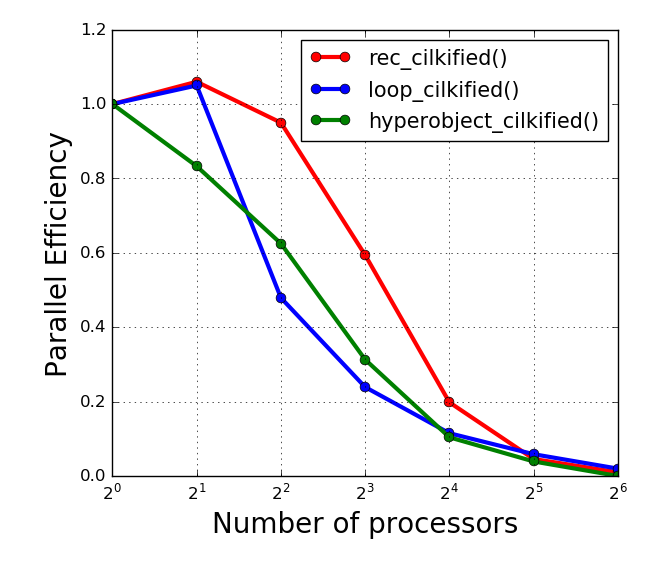
\includegraphics[scale=0.45]{ncores_scaling.png}
\caption{Parallel efficiency vs number of processors, Array size = $10^6$, COARSENESS = 50}
\end{figure}
%
\section*{Sensitivity to COARSENESS}
\noindent For this experiment, the array size was fixed at $10^8$ and was run on all 24 cores of a single Comet compute node. COARSENESS was varied from 1 to $10^8$ in powers of 10. 
%
\begin{figure}[h]
\centering
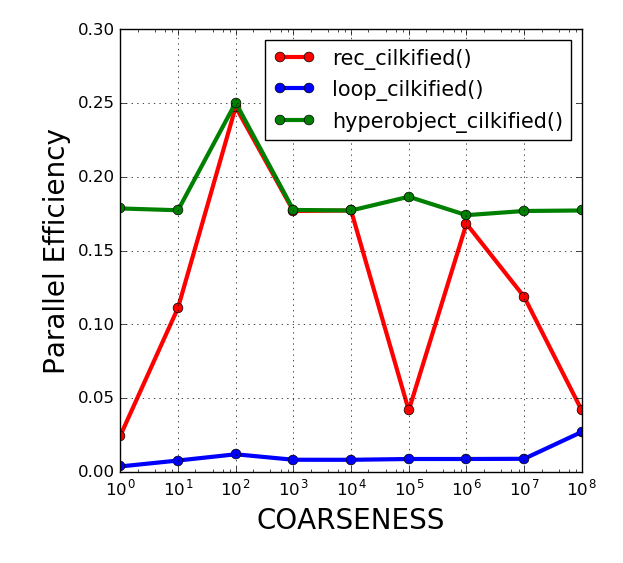
\includegraphics[scale=0.5]{coarseness_sensitivity.png}
\caption{Parallel efficiency vs COARSENESS, Array size = $10^8$, NCores = 24}
\end{figure}
%
\section*{Best performing dot-product code}
\noindent From the different scaling studies presented above, Fig. 1 shows that with increasing number of cores (and therefore spawned threads), the performance goes down. Thus, the performance is never truly a function of how much computational resources I have at my disposal. On the other hand, increasing array sizes is a very real world phenomenon, and it should be the primary metric on which to judge performance. For large array sizes, \texttt{rec\_cilkified} and \texttt{hyperboject\_cilkified} have nearly similar parallel efficiency in Fig. 2. So any of these two might be a good candidate. Now, coming to COARSENESS, we see from Fig. 3, that \texttt{rec\_cilkified} is much more sensitive than \texttt{hyperobject\_cilkified}. That means that the former is amenable to easy tuning.\\

\noindent On the basis of the above insights, I would use the following parameters for the best-performing dot product code:
%
\begin{itemize}
\item Function: \texttt{rec\_cilkified()}
\item COARSENESS: 100
\end{itemize}
%
\begin{figure}[h]
\centering
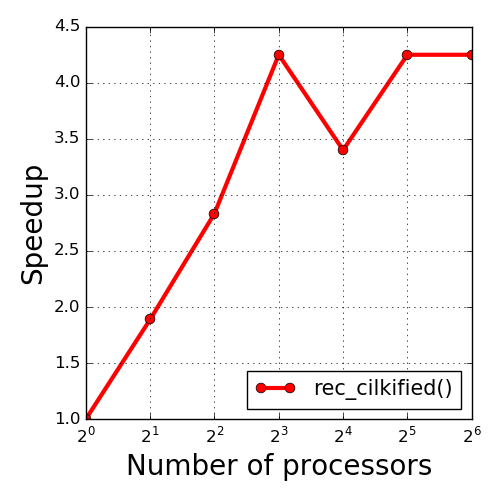
\includegraphics[scale=0.5]{best_dot_prod.png}
\caption{Speedup vs number of cores with \texttt{rec\_cilkified}, Array size = $10^6$, COARSENESS = 100}
\end{figure}
%
\noindent Clearly, this does not enjoy linear speedup. Beyond 16 processors, the speedup saturates, because the threads are no longer in truly shared memory and span different Comet nodes (thus possibly doing hyperthreading behind the scenes). That is a trivial bottleneck. But the speedup also falls (and drastically so) from 8 to 16 processors, which are all within the same node. (I still can't think of a good reason why this happens)

\section*{Cilkscreen and Cilkview}
\noindent It is worth mentioning that of the three methods, \texttt{hyperobject\_cilkified} is the most \textit{stable}, in the sense that it handles data races very efficiently. On the other end of the spectrum is \texttt{loop\_cilkified} which starts producing incorrect results more often than not, as input array size grows beyond $10^5$. I ran a test with $n = 10^4$, COARSENESS = 100 on 10 cores of a single node and ntoticed data race reports only for \texttt{loop\_cilkified}.
%
\newpage
\begin{figure}[h!]
\flushleft
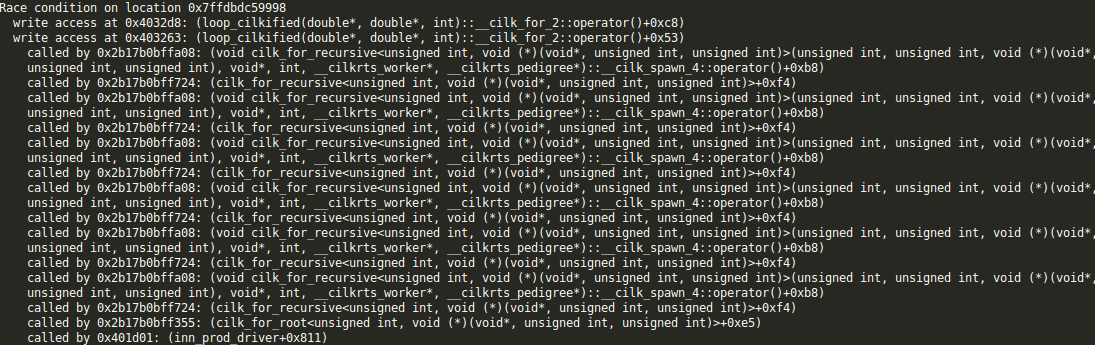
\includegraphics[scale=0.45]{race_loop_cilkified.png}
\caption{Race conditions in \texttt{loop\_cilkified}}
\end{figure}
%
\noindent I used cilkview to estimate the parallelism (of the parallel region only). The estimated parallel efficiency in Fig. 6 matches the one from \texttt{hyperobject\_cilkified} from Fig.2. We can conjecture (albeit hardly rigorous) that the built in reducer hyperobject is indeed a very stable model.
\begin{figure}[h]
\flushleft
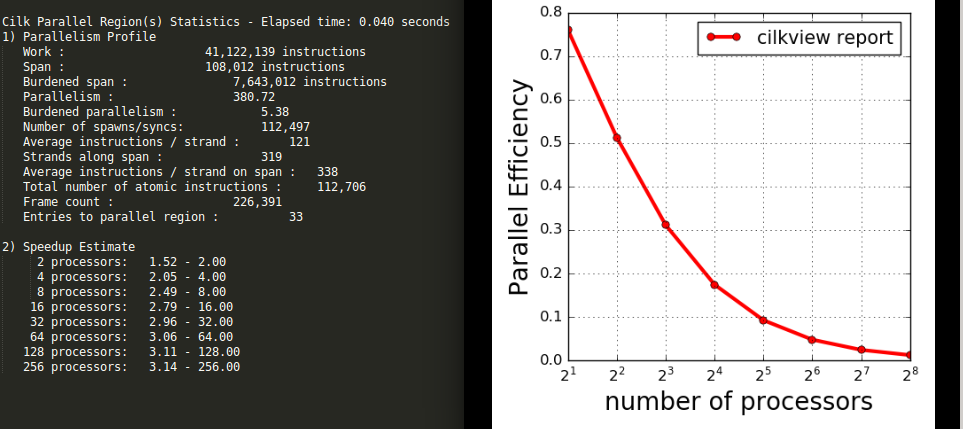
\includegraphics[scale=0.5]{ncores_scaling_cilkview.png}
\caption{Empirical parallelism as reported by cilkview}
\end{figure}
%
\end{document}